\section{Formal Analysis Using Alloy}
Alloy is a specification language for describing, designing, and verifying the behavior of complex systems.
The language is based on first-order logic, and has a mathematical foundation that allows for automated reasoning
about the correctness of designs.
Once a model has been defined, it will be analyzed using a tool that supports Alloy. This tool can automatically check
whether the model satisfies the specified constraints and properties, and can also be used to explore the space of
possible behaviors to find designs that meet the desired criteria.

\subsection{Objectives of the analysis}
The main goal of the formal analysis is to formally describe the domain and properties of the system to be.
This goal is reachable modelling and formally representing the following entities:
\begin{itemize}
    \item reservations
\end{itemize}

\subsubsection{Reservation Model}
The Alloy model for verifying reservations of charging points includes abstractions
for the entities involved in a reservation, such as charging points, electric vehicles, and reservation times.
It also includes constraints on the relationships between these entities, such as the fact that a charging point
can be reserved by one vehicle at a time, or that a vehicle can be charged by one charging point at a time.

\lstinputlisting[language=C, basicstyle=\ttfamily\footnotesize]{src/alloy/reservationModel.als}
\begin{figure}[H]
    \centering
    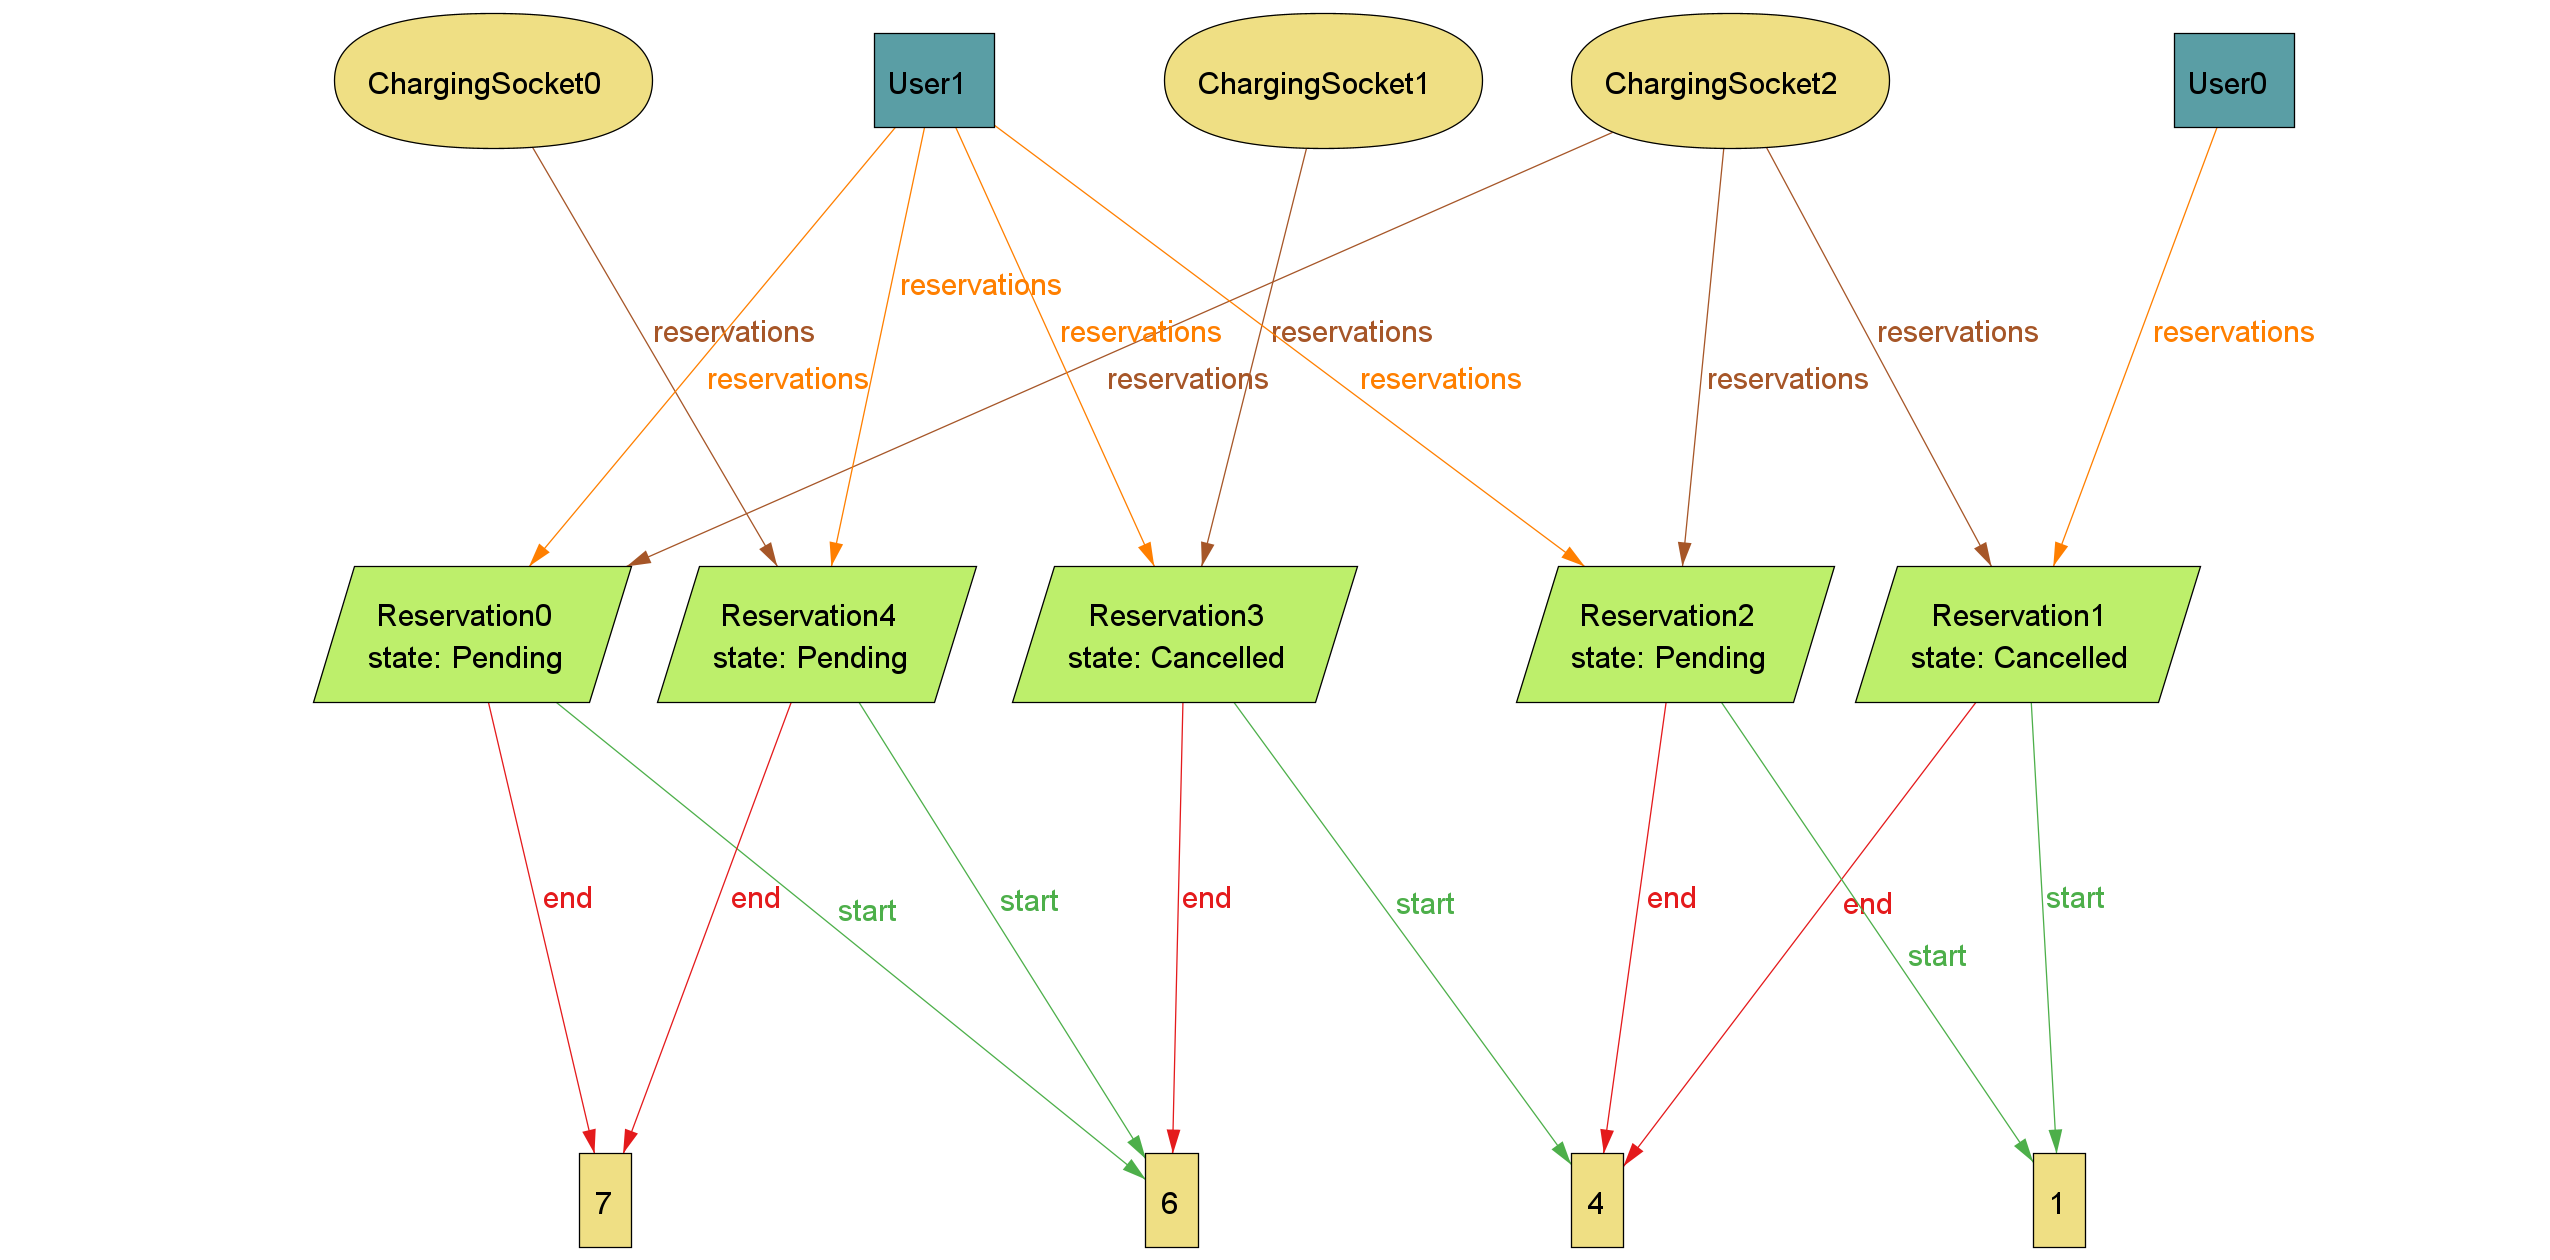
\includegraphics[width=1\textwidth]{src/alloy/reservationModel.png}
\end{figure}
\begin{figure}[H]
    \centering
    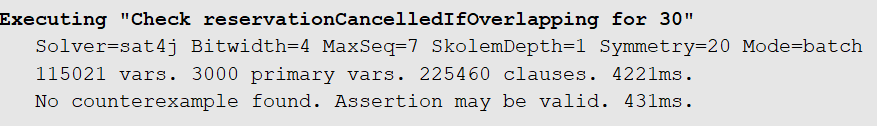
\includegraphics[width=1\textwidth]{src/alloy/reservationModel_assertion.png}
\end{figure}

\subsubsection{A title for the second model}
Description for the second model
\lstinputlisting[language=C, basicstyle=\ttfamily\footnotesize]{src/alloy/secondmodel.als}
\begin{figure}[H]
    \centering
    %\includegraphics[width=1\textwidth]{alloy/secondmodel.png} the image of the world
\end{figure}

\subsubsection{Dynamic Modeling of reservations}
Here a dynamic model of reservation with user that reserve CPs, no overlapping of reservation and the fact that a user can reserve a CP at a time
\dots
